\documentclass[tikz,border=10pt]{standalone}
\usetikzlibrary{calc}
\begin{document}
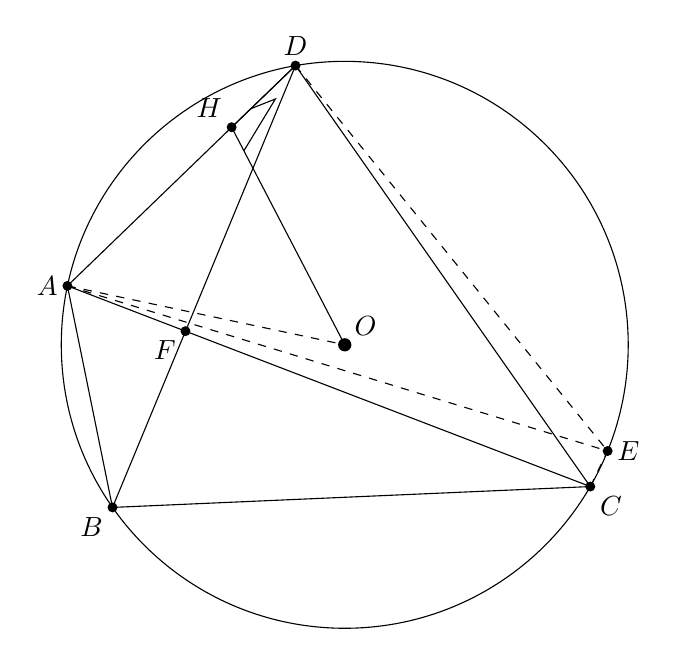
\begin{tikzpicture}[scale=1.2]
% Circle center and radius
\coordinate (O) at (0,0);
\def\rad{3}
% Points on circle
\coordinate (D) at (100:\rad);
\coordinate (A) at (168:\rad);
\coordinate (B) at (215:\rad);
\coordinate (C) at (330:\rad);
\coordinate (E) at (338:\rad);
% Intersection points
\coordinate (F) at (intersection of A--C and B--D);
\coordinate (H) at ($(D)!0.28!(A)$);
% Circle
\draw (O) circle (\rad);
% Solid lines
\draw (A) -- (B) -- (C) -- (D) -- cycle;
\draw (A) -- (C);
\draw (B) -- (D);
\draw (D) -- (H);
\draw (O) -- (H);
% Dashed lines
\draw[dashed] (A) -- (O);
\draw[dashed] (A) -- (E);
\draw[dashed] (D) -- (E);
\draw[dashed] (C) -- (E);
% Right angle mark at H (between DH and OH)
\draw ($(H)!8pt!(D)$) -- ($($(H)!8pt!(D)$)!8pt!90:(O)$) -- ($(H)!8pt!(O)$);
% Points
\fill (O) circle (2pt);
\foreach \p in {A,B,C,D,E,F,H} \fill (\p) circle (1.5pt);
% Labels
\node[above] at (D) {$D$};
\node[above left] at (H) {$H$};
\node[left] at (A) {$A$};
\node[below left] at (B) {$B$};
\node[below right] at (C) {$C$};
\node[right] at (E) {$E$};
\node[below left] at (F) {$F$};
\node[above right] at (O) {$O$};
\end{tikzpicture}
\end{document}
